\documentclass[12pt, a4paper, simple]{eskdtext}

\usepackage{config/main.env}
\usepackage{config/report.env}
\usepackage{styles/listing}
\usepackage{styles/lists}
\usepackage{styles/SectionMargins}
\usepackage{styles/table}
\usepackage{styles/TableOfContent}
\usepackage{styles/url}

\begin{document}
  \begin{ESKDtitlePage}
  \ESKDstyle{empty}
  \begin{center}
    \envReportMinistr \\
    \envReportEducation \\
    \envReportUniversity \\
    \envReportCathedra \\
  \end{center}

  \vfill

  \begin{center}
    Тема: <<\envReportTitle>>
  \end{center}

  \vfill

  \begin{center}
    Отчёт лабораторной работы №\envReportLabNumber \\
    по дисциплине \envReportSubject \\
  \end{center}

  \vfill

  \begin{flushright}
    \begin{minipage}[t]{7cm}
      Выполнил: \\
      \envReportStudentInfo \\
      \hspace{0pt} \\
      Проверил: \\
      \envReportTeacherInfo \\
    \end{minipage}
  \end{flushright}

  \vfill

  \begin{center}
    \envReportCity~\ESKDtheYear
  \end{center}
\end{ESKDtitlePage}


  % = = = = = = = = = = = = = = = =
  \ESKDstyle{empty}
  \begin{center}
    \textbf{Отчёт лабораторной работы №\envReportLabNumber}
  \end{center}

  \paragraph{} \textbf{Тема}: <<\envReportTitle>>

  \paragraph{} \textbf{Цель}:
  Знакомство с App Engine, Pub/Sub.

  \paragraph{} \textbf{Что нужно сделать}:

  Напишите микросервис MS3, реализующий функциональность биллинговой системы,
  в которую приложение MS2 будет отправлять данные каждый раз, когда происходит «Регистрация события». 

  Связь между двумя сервисами – с использованием Pub/Sub.

  Задача микросервиса MS3 – обработать/оценить полученные данные (случайным образом, не надо реальный биллинг строить)
  и вернуть в MS2 результат: положительный или отрицательный – разрешено действие или нет.
  MS2 в зависимости от этого должно произвести некие действия, например, отменить заказ или удалить товар из корзины.

  \paragraph{} \textbf{Ход работы}:

  Смотрим видео на YouTube по работе с PubSub \cite{YouTube_PubSub}.

  \textbf{Создание темы PubSub (MS2 to MS3 и MS3 to MS2)}

  Заходим на сайт Google Cloud Console \cite{GoogleCloudConsole} (см. рисунок~\ref{fig:1}).

  Menu > Pub/Sub > Topics \cite{GoogleCloudPubSubTopic} (см. рисунок~\ref{fig:1}).

  \begin{figure}[!h]
    \centering
    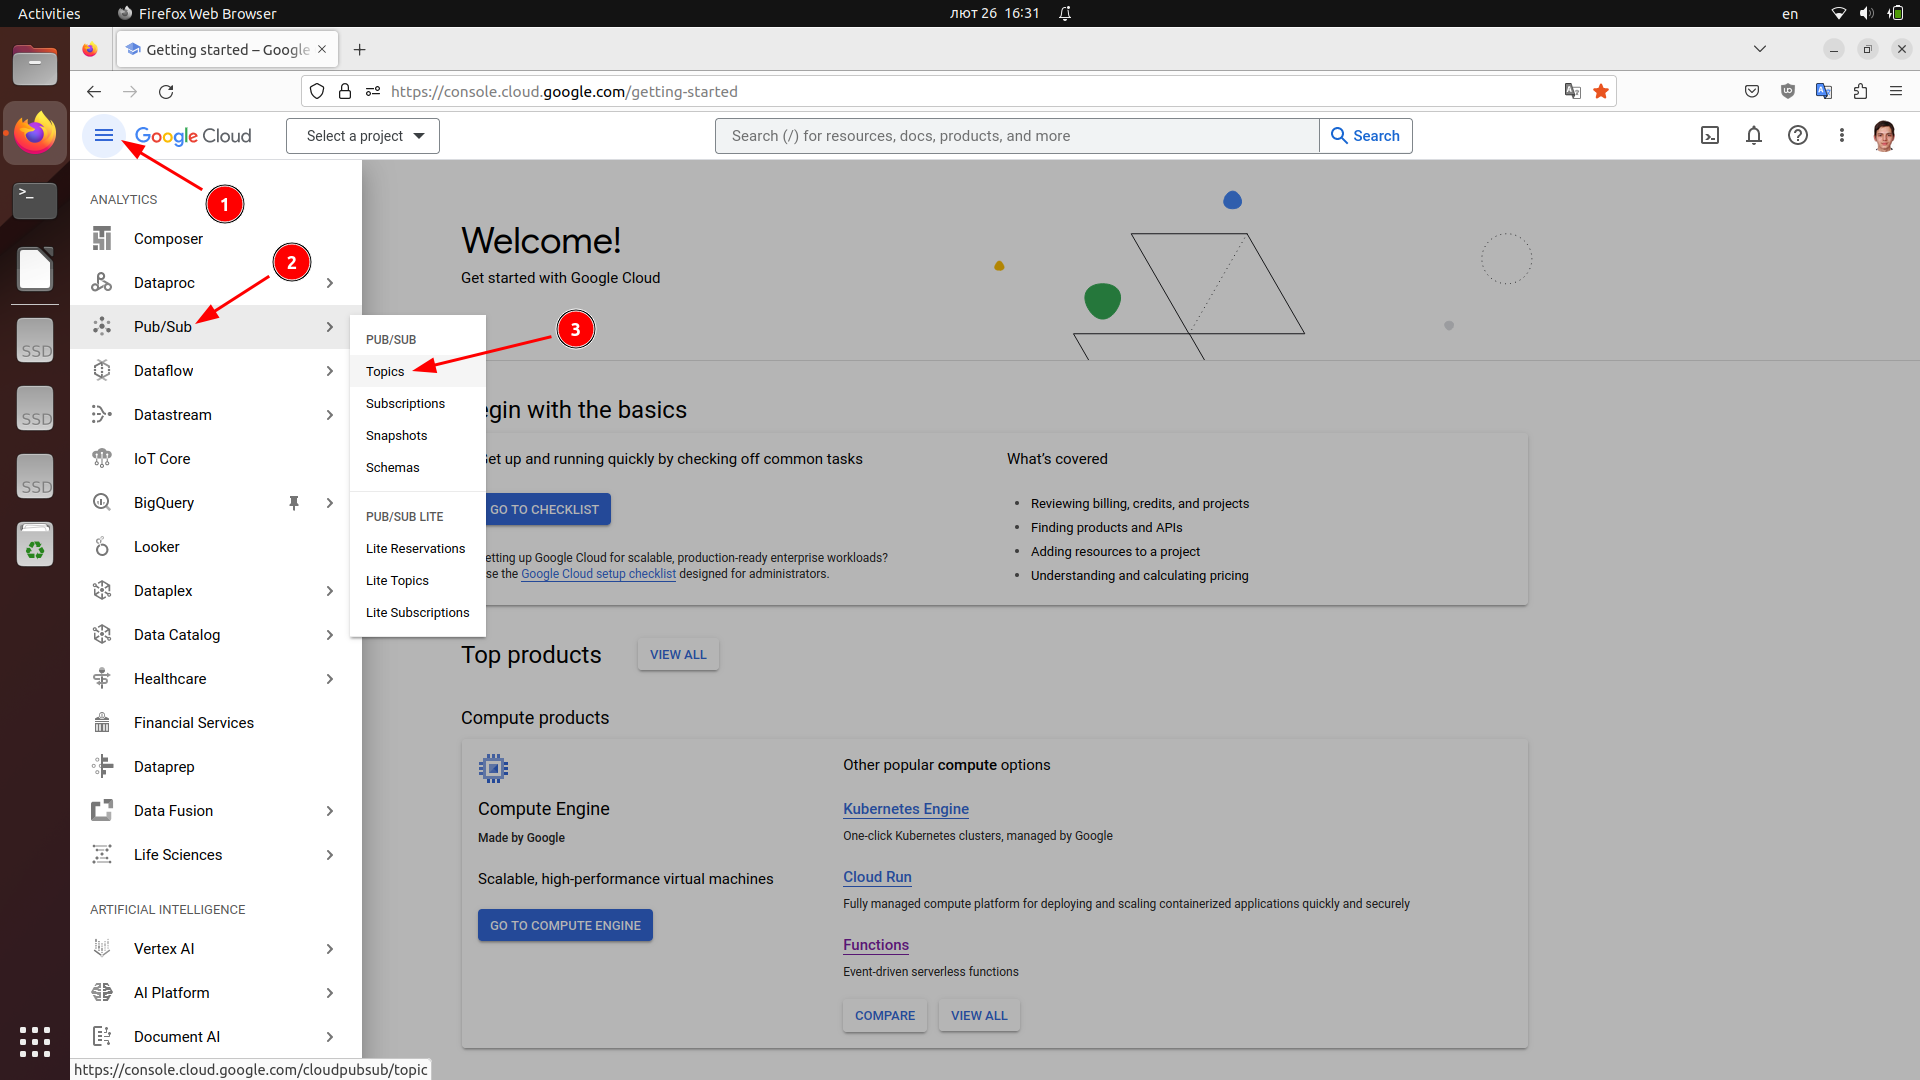
\includegraphics[width=11cm]
    {images/2023-02-26_16-32-28.png}
    \caption{\_}
    \label{fig:1}
  \end{figure}

  Создаем тему для MS2 to MS3...

  Жмём <<CREATE TOPIC>> (см. рисунок~\ref{fig:2}).

  Topic ID: \underline{rsiot-po4-190333-ms2-to-ms3-pubsub-topic} (см. рисунок~\ref{fig:2}).
  
  Жмём <<CREATE TOPIC>> (см. рисунок~\ref{fig:2}).

  Создаем тему для MS3 to MS2...

  Жмём <<CREATE TOPIC>> (см. рисунок~\ref{fig:3}).

  Topic ID: \underline{rsiot-po4-190333-ms3-to-ms2-pubsub-topic} (см. рисунок~\ref{fig:3}).
  
  Жмём <<CREATE TOPIC>> (см. рисунок~\ref{fig:3}).

  \begin{figure}[!h]
    \centering
  
    \begin{minipage}{0.49\textwidth}
      \centering
  
      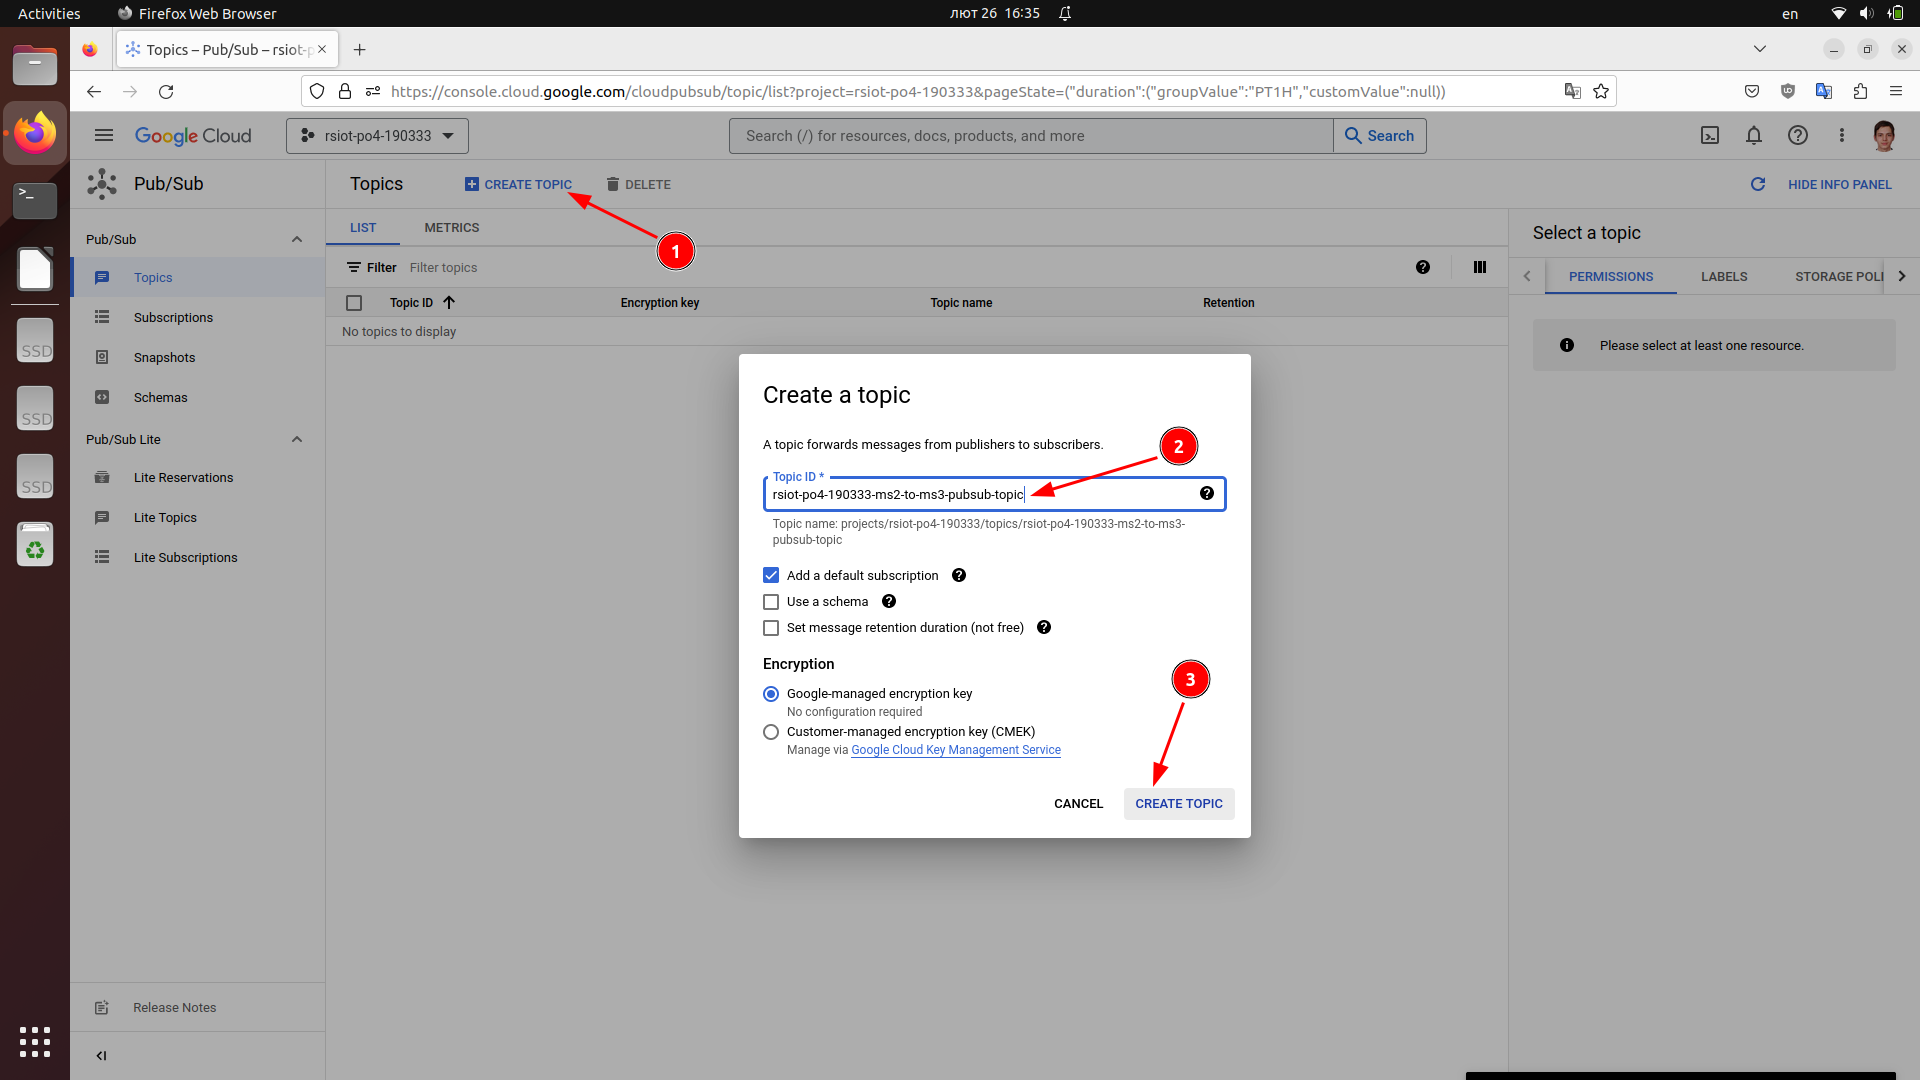
\includegraphics[height=5cm]
      {images/2023-02-26_16-36-09.png}
  
      \caption{\_}
  
      \label{fig:2}
    \end{minipage}
    \begin{minipage}{0.49\textwidth}
      \centering
  
      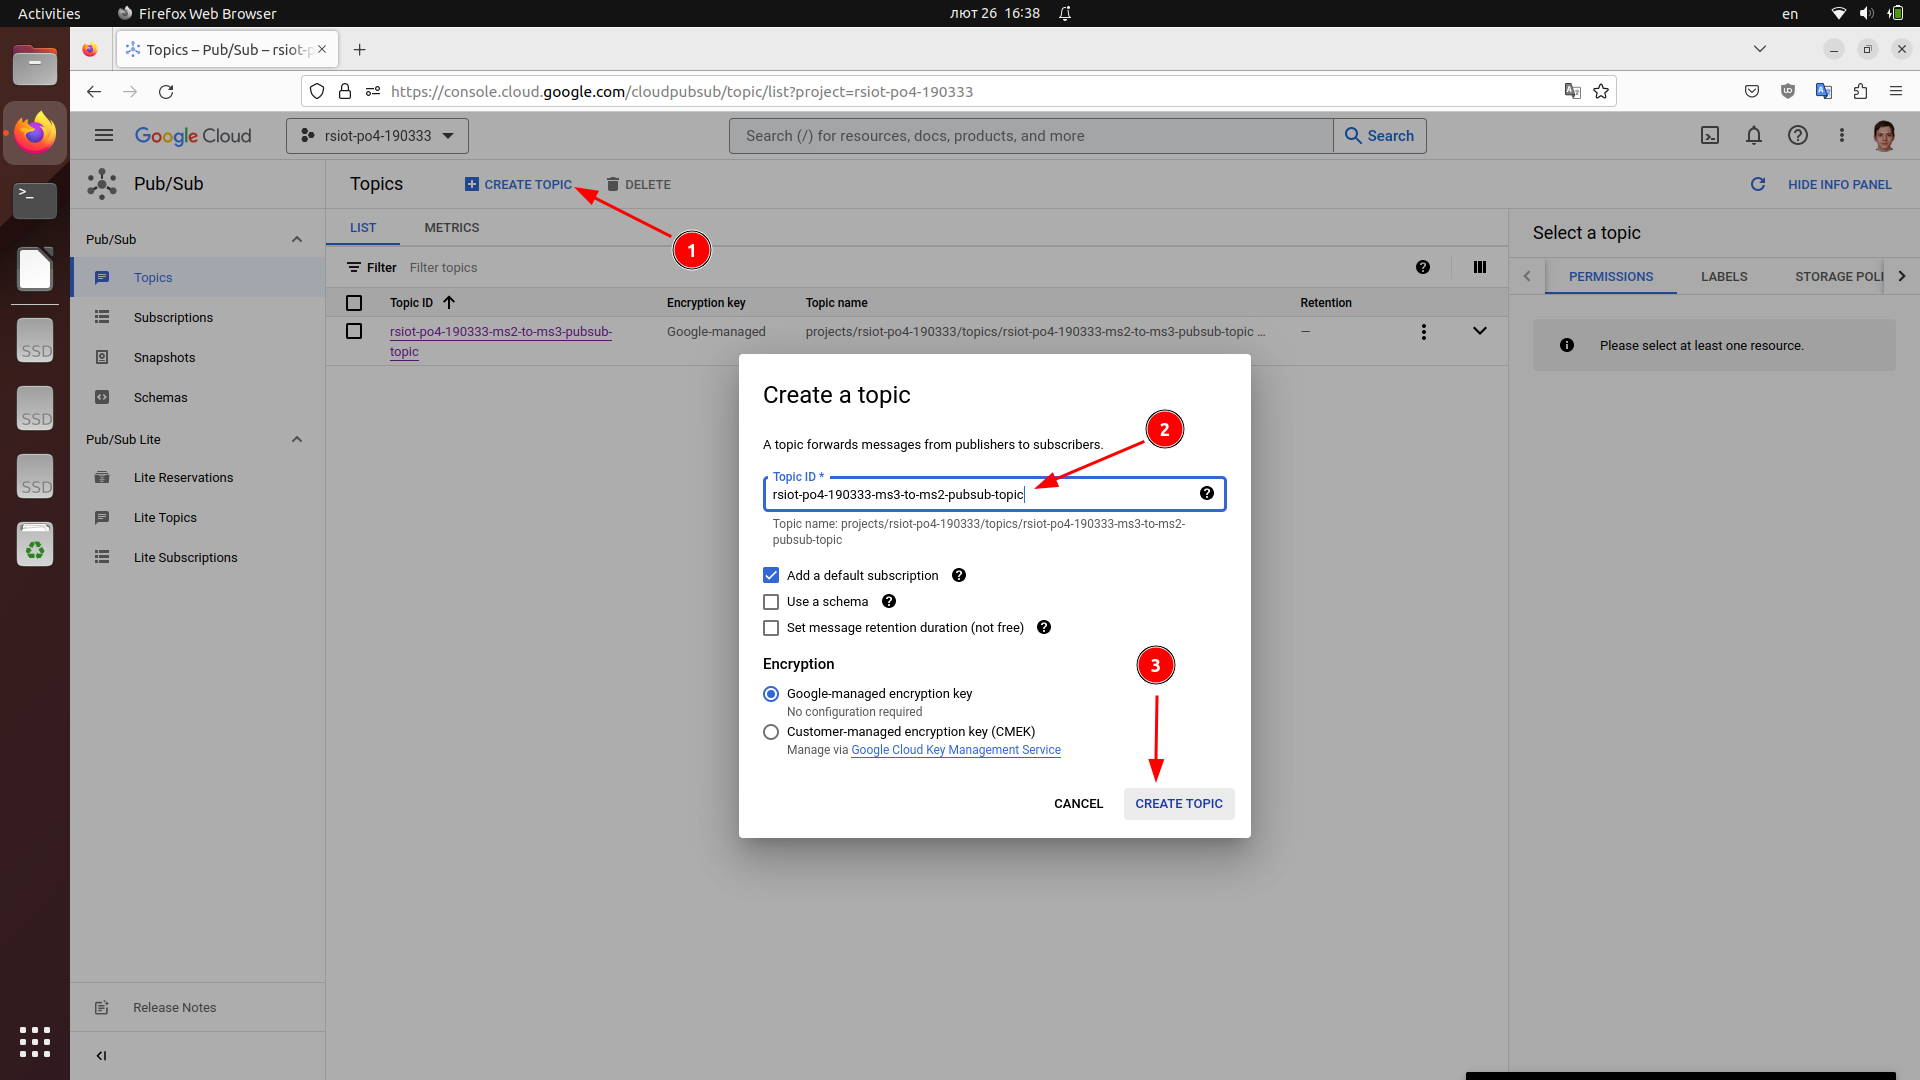
\includegraphics[height=5cm]
      {images/2023-02-26_16-38-42.png}
  
      \caption{\_}
  
      \label{fig:3}
    \end{minipage}
  \end{figure}

  \newpage

  При создании тем у нас создались подписчики \cite{GoogleCloudPubSubSubscriptions} (см. рисунок~\ref{fig:4}):
  \begin{itemize}
      \item \underline{rsiot-po4-190333-ms2-to-ms3-pubsub-topic-sub}
      \item \underline{rsiot-po4-190333-ms3-to-ms2-pubsub-topic-sub}
  \end{itemize}

  \begin{figure}[!h]
    \centering
    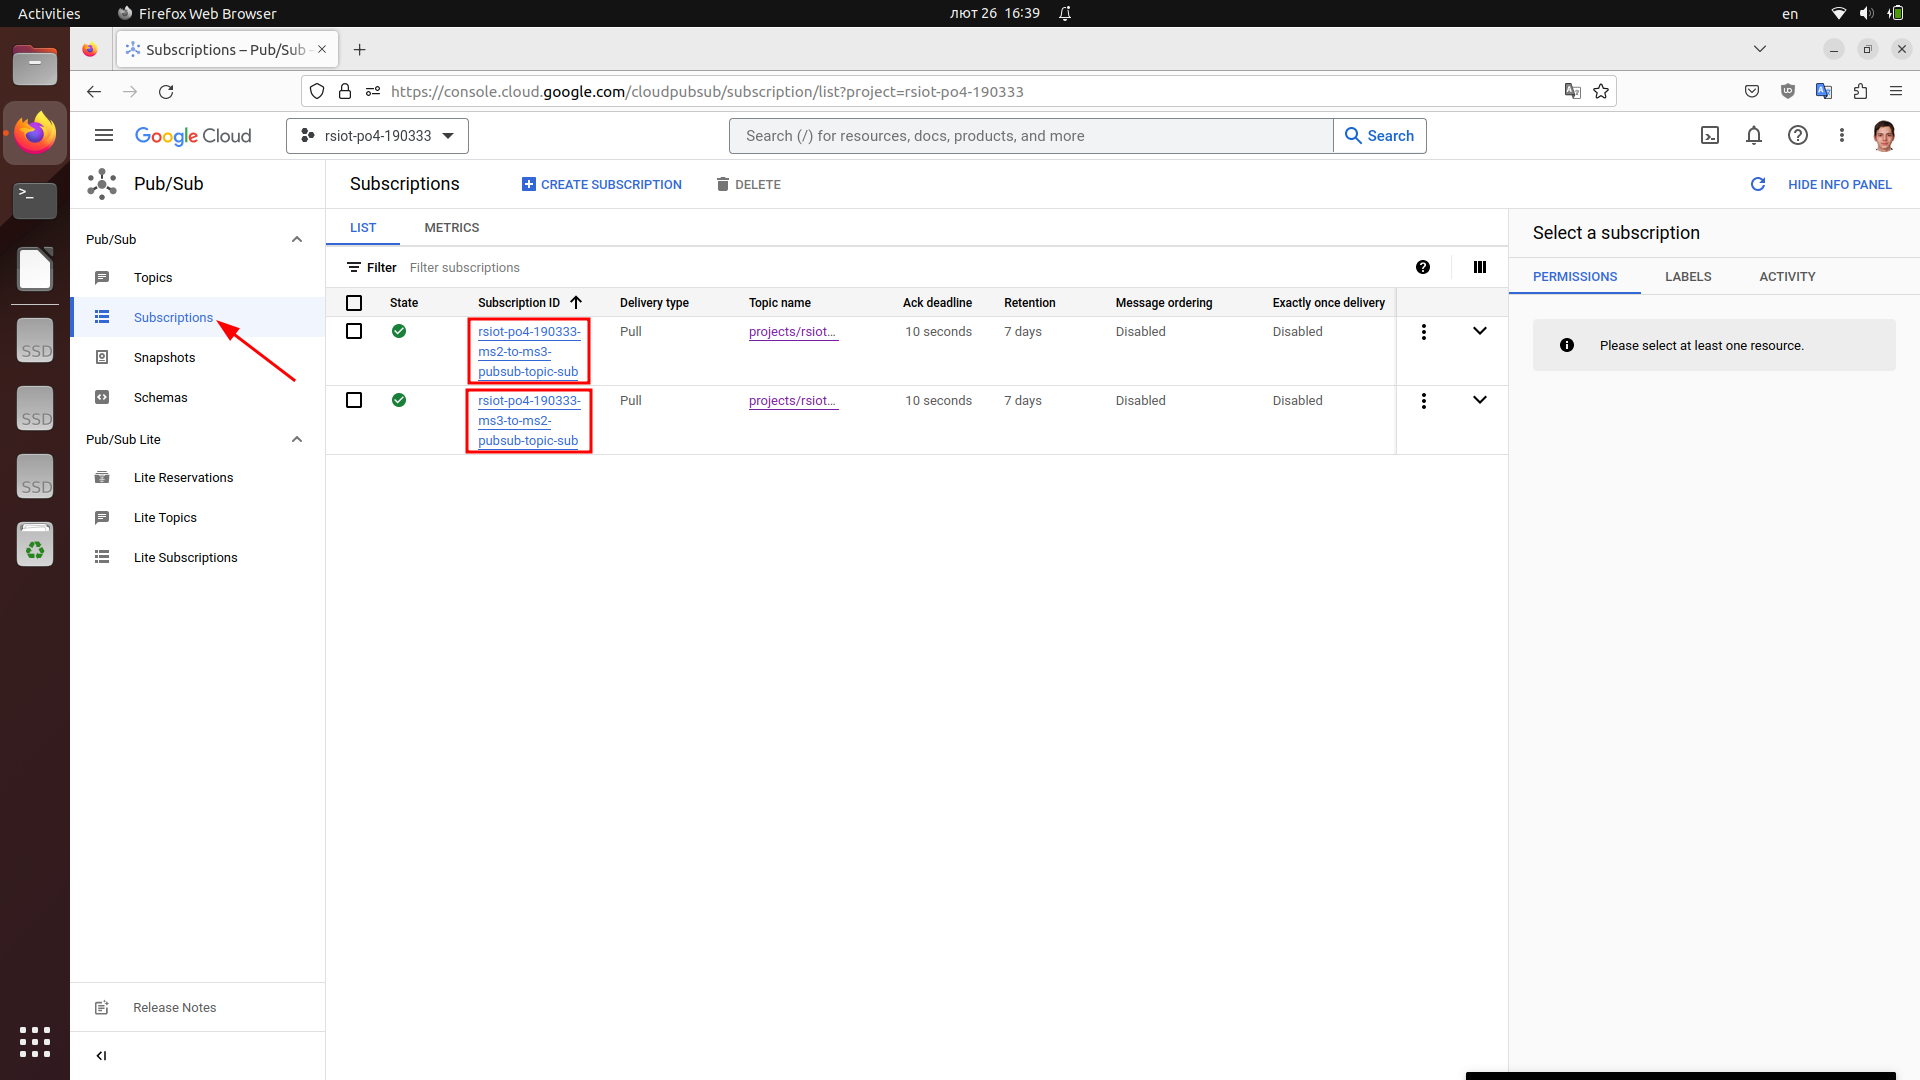
\includegraphics[width=11cm]
    {images/2023-02-26_16-39-41.png}
    \caption{\_}
    \label{fig:4}
  \end{figure}

  \textbf{Создание сервис аккаунта}

  Заходим на сайт Google Cloud Console \cite{GoogleCloudConsole} (см. рисунок~\ref{fig:5}).

  Menu > IAM \& Admin > Service Accounts \cite{GoogleCloudServiceAccount} (см. рисунок~\ref{fig:5}).

  \begin{figure}[!h]
    \centering
    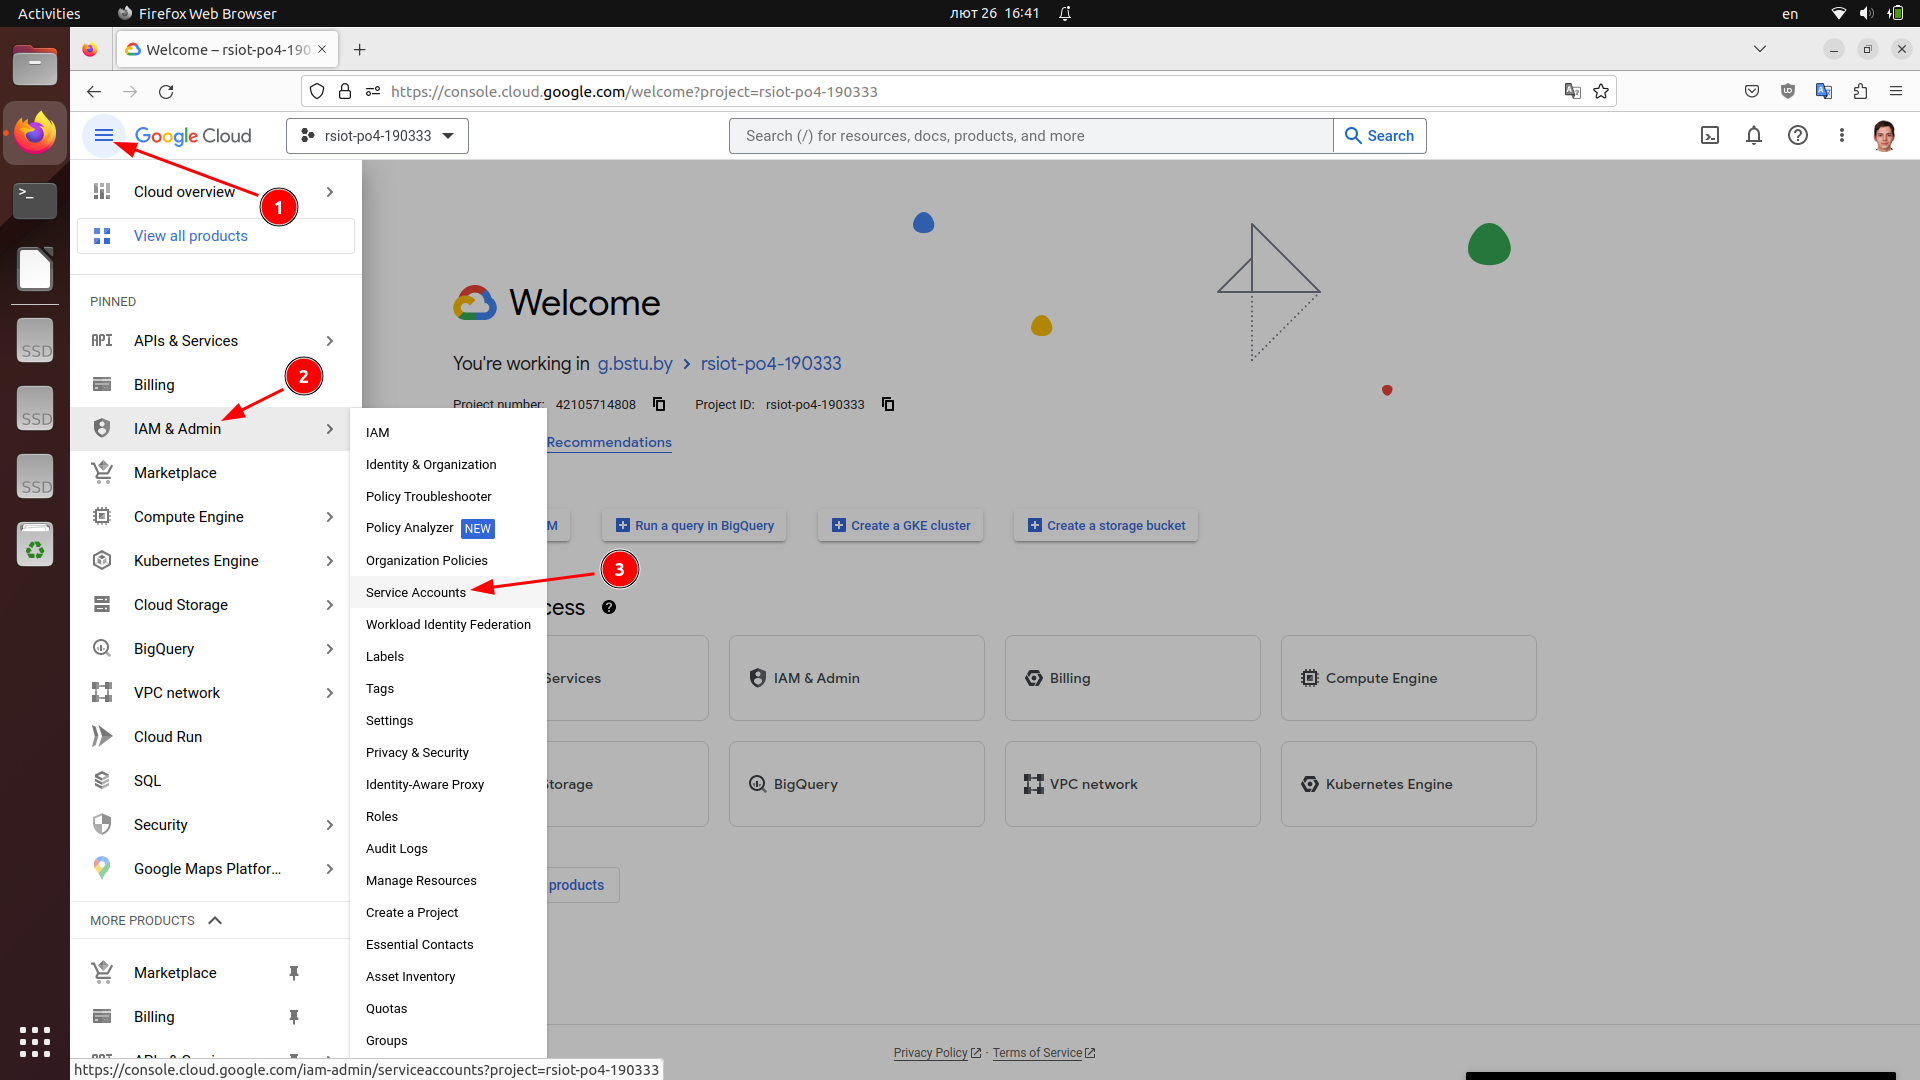
\includegraphics[width=11cm]
    {images/2023-02-26_16-41-55.png}
    \caption{\_}
    \label{fig:5}
  \end{figure}

  \newpage
  Жмём <<CREATE SERVICE ACCOUNT>> (см. рисунок~\ref{fig:6}).

  \begin{figure}[!h]
    \centering
    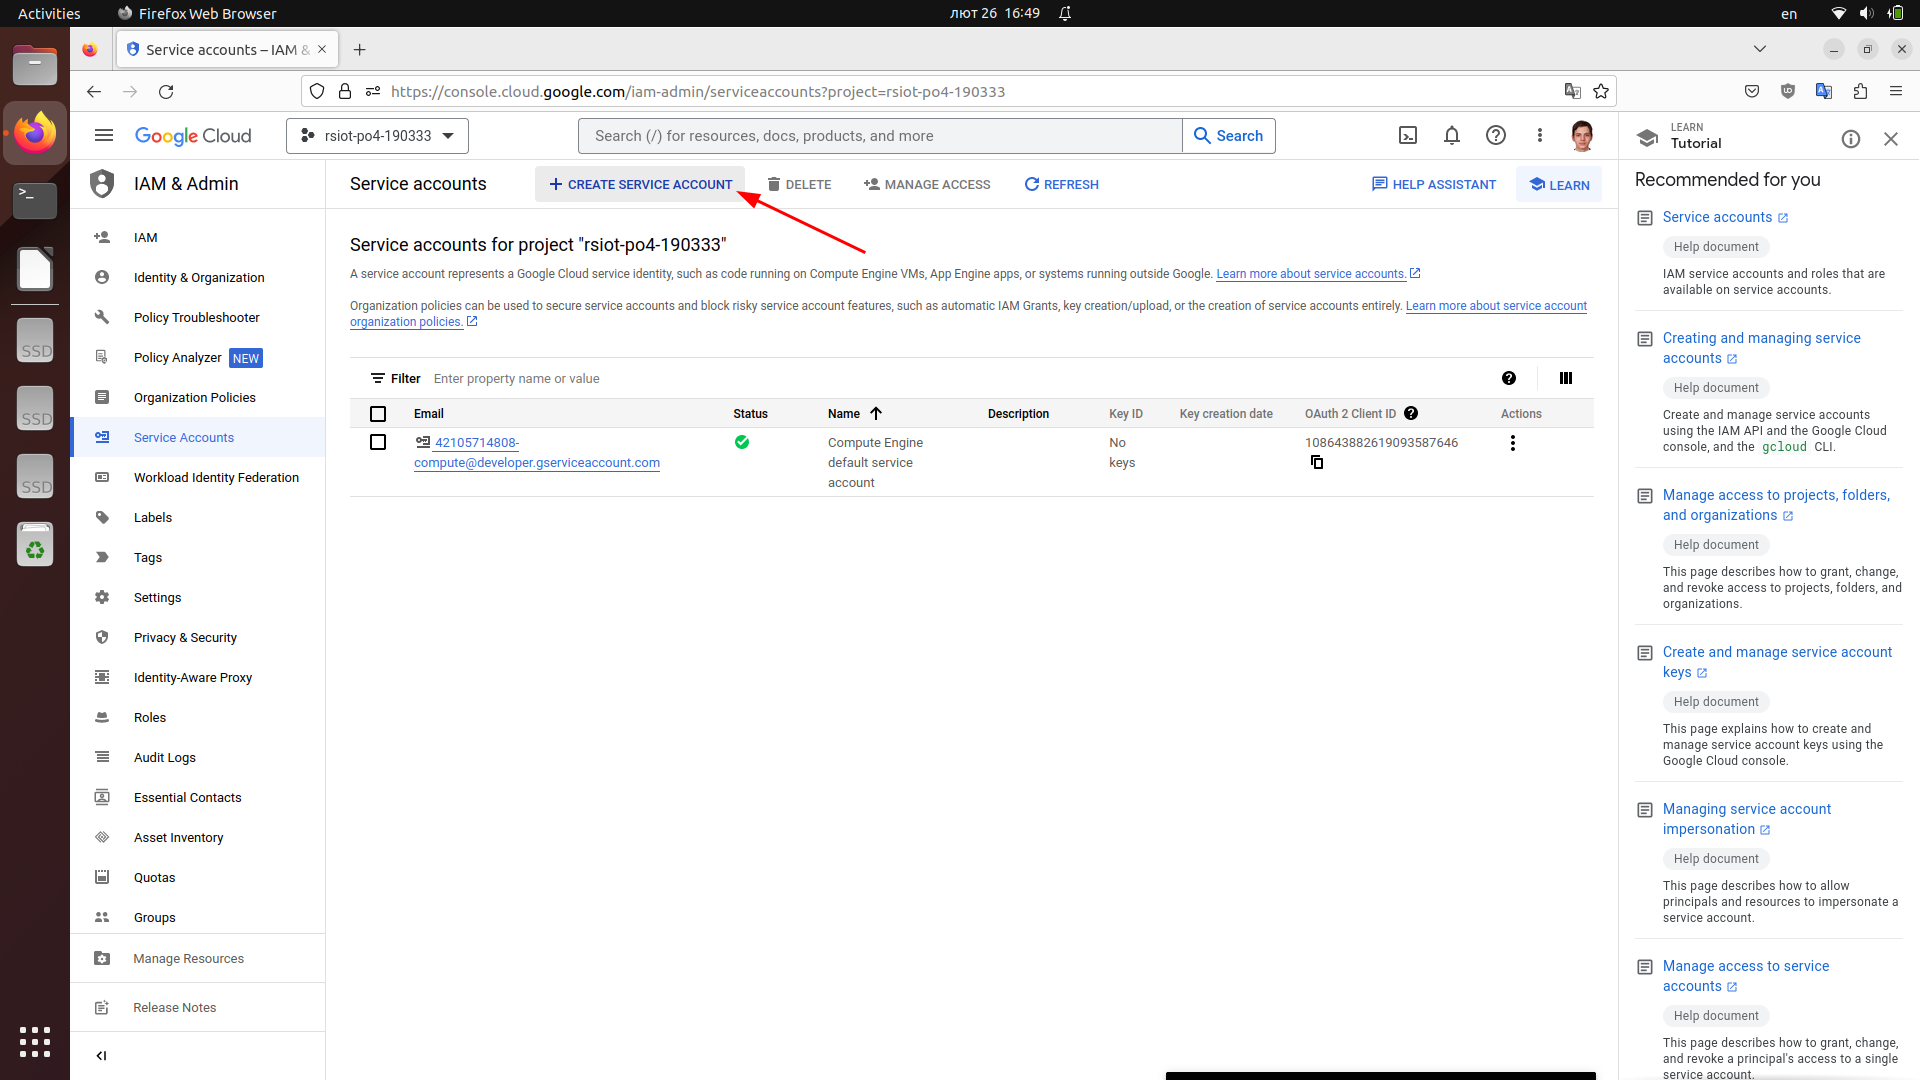
\includegraphics[width=11cm]
    {images/2023-02-26_16-49-46.png}
    \caption{\_}
    \label{fig:6}
  \end{figure}

  Service account ID: \underline{ms2-to-ms3-service-account} (см. рисунок~\ref{fig:7}).

  Жмём <<CREATE AND CONTINUE>> (см. рисунок~\ref{fig:7}).

  \begin{figure}[!h]
    \centering
    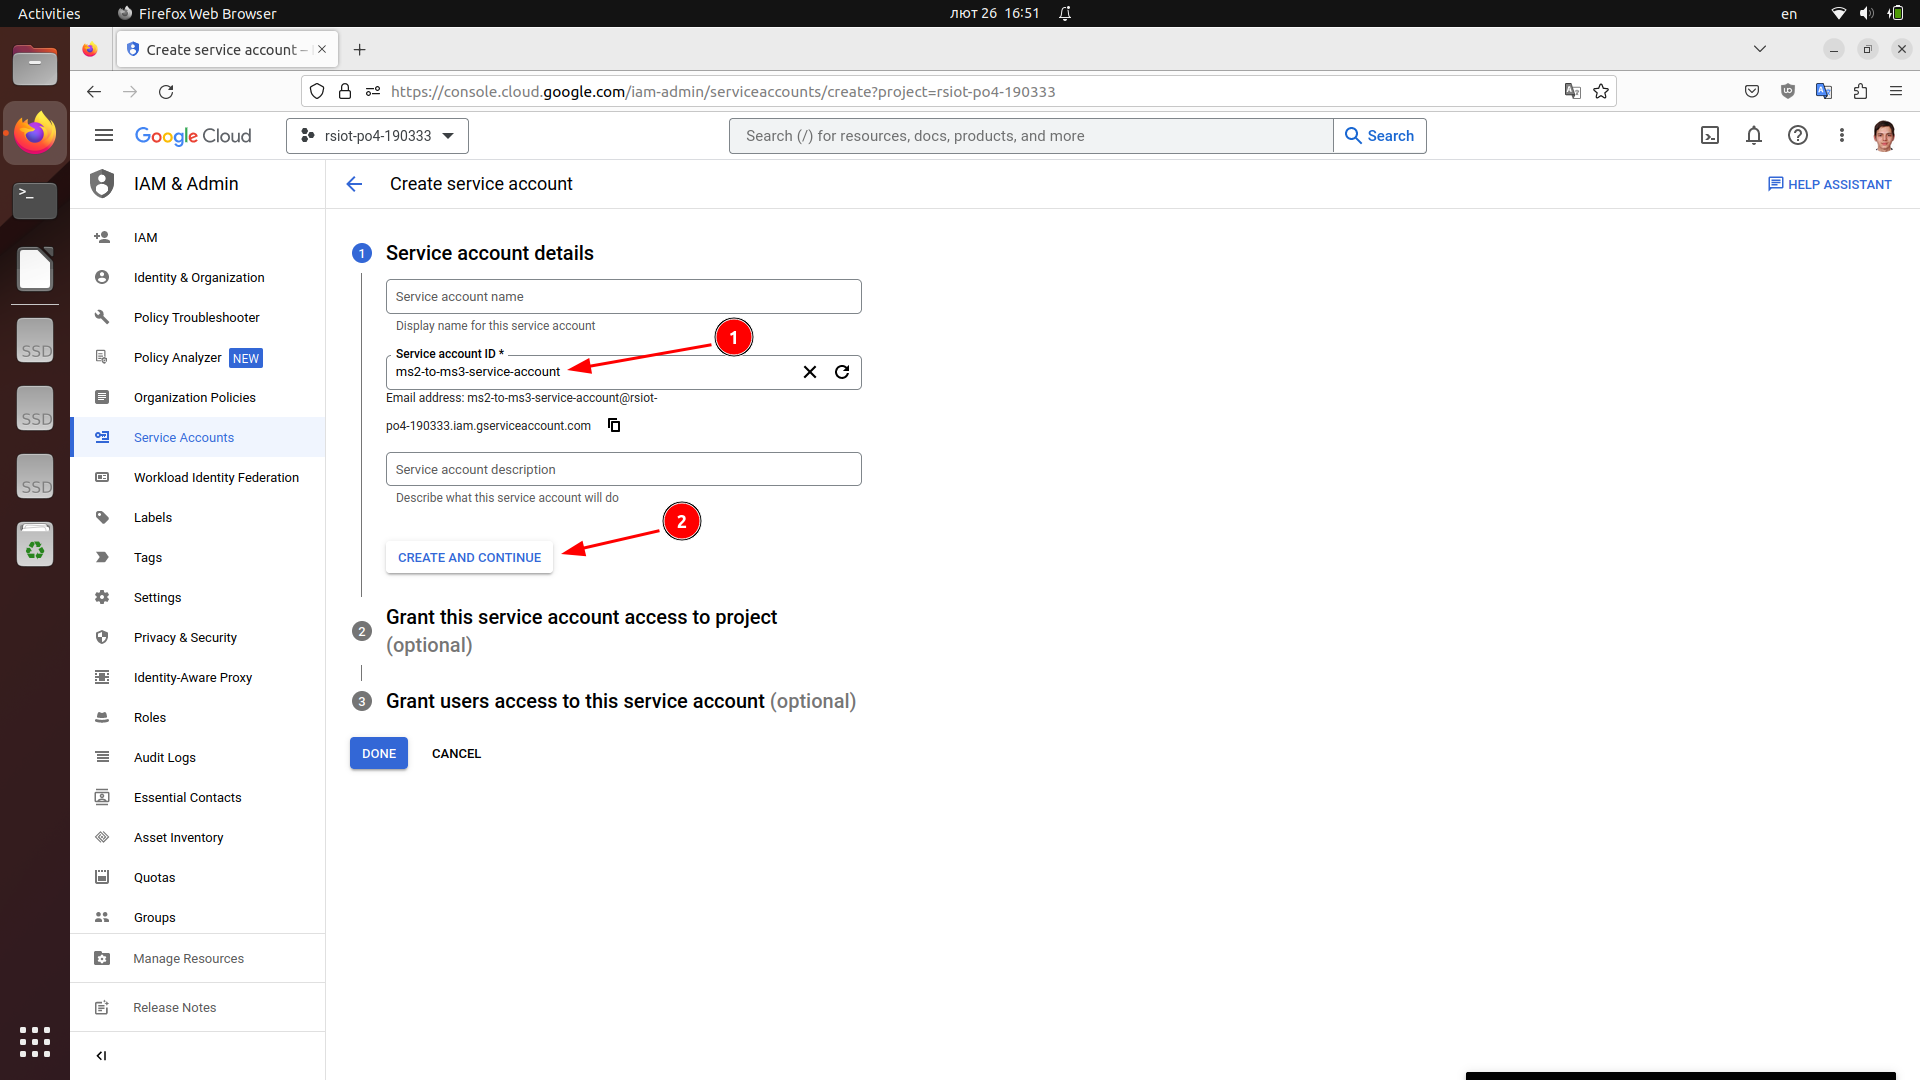
\includegraphics[width=11cm]
    {images/2023-02-26_16-52-22.png}
    \caption{\_}
    \label{fig:7}
  \end{figure}

  Select a role > Pub/Sub > Pub/Sub Admin > CONTINUE (см. рисунок~\ref{fig:8}).

  \begin{figure}[!h]
    \centering
    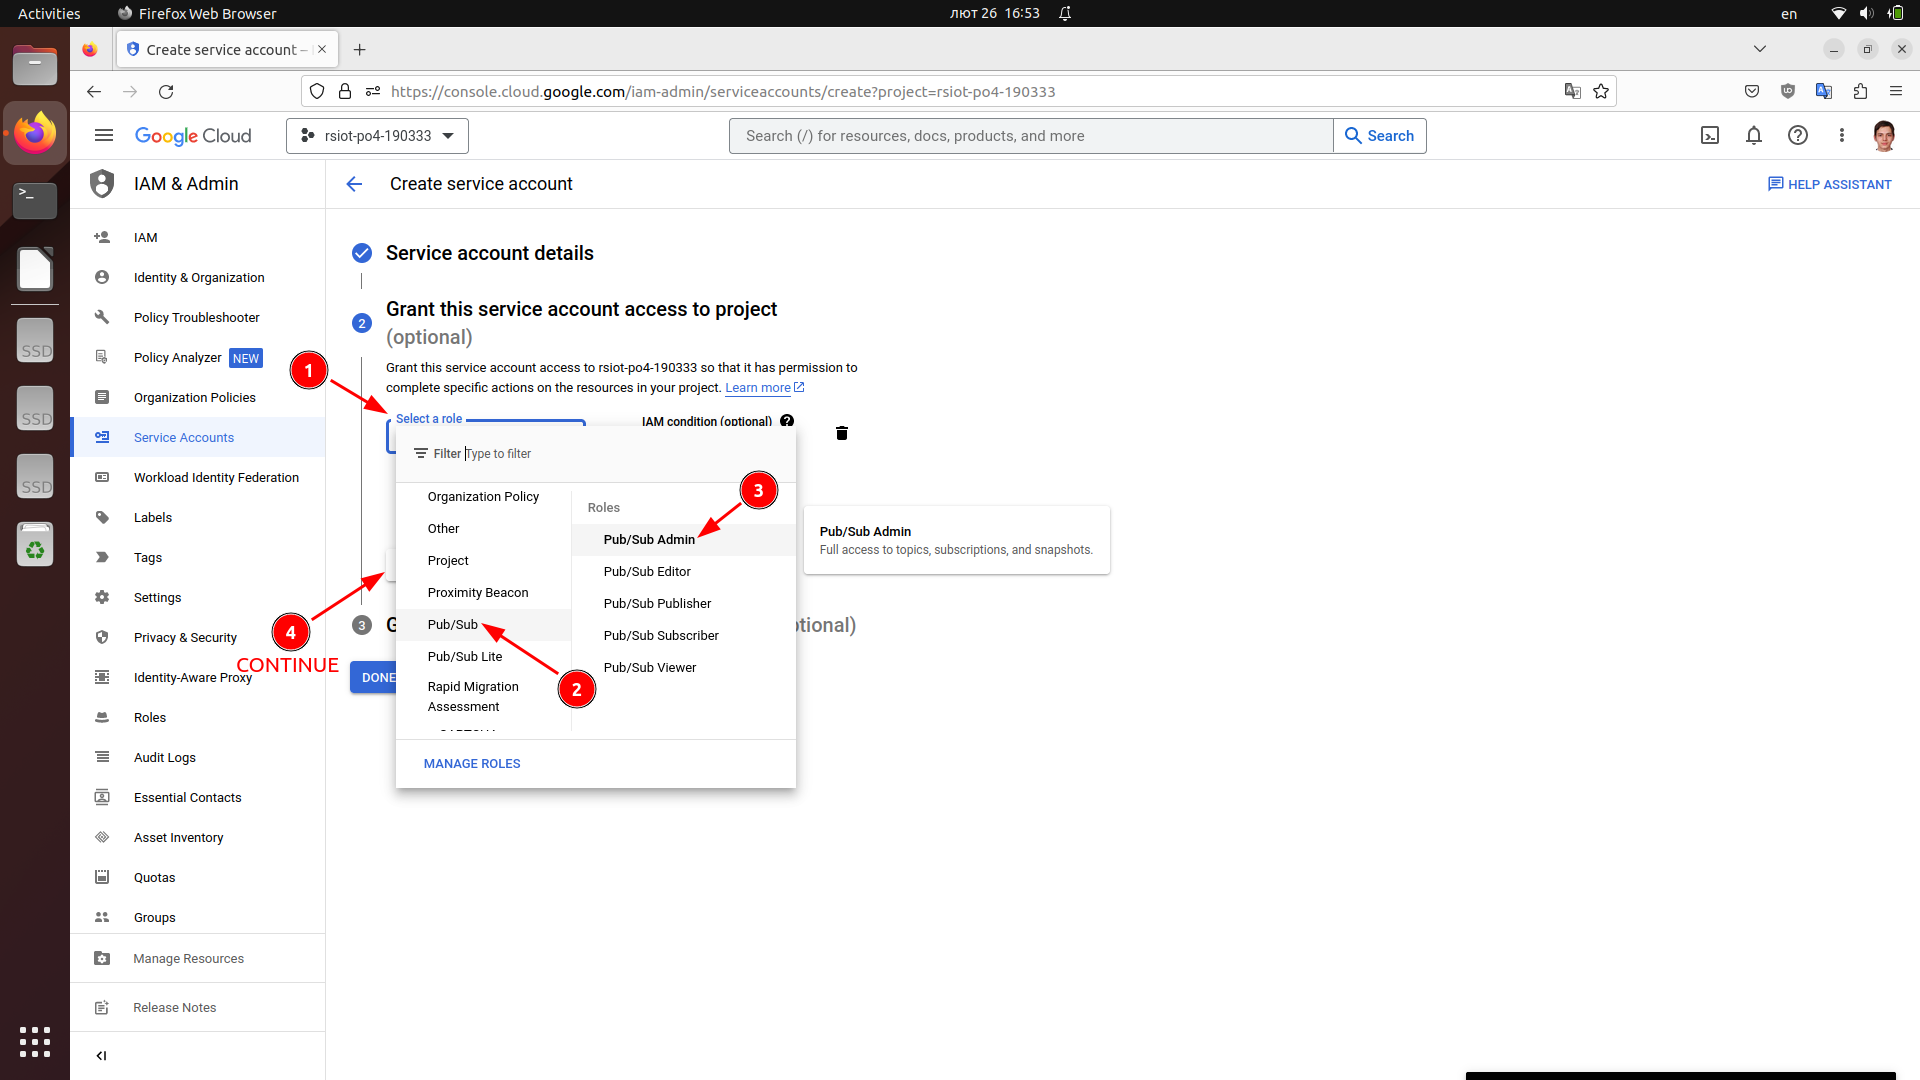
\includegraphics[width=11cm]
    {images/2023-02-26_16-55-33.png}
    \caption{\_}
    \label{fig:8}
  \end{figure}

  \newpage
  Жмём <<Done>> (см. рисунок~\ref{fig:8}).

  \begin{figure}[!h]
    \centering
    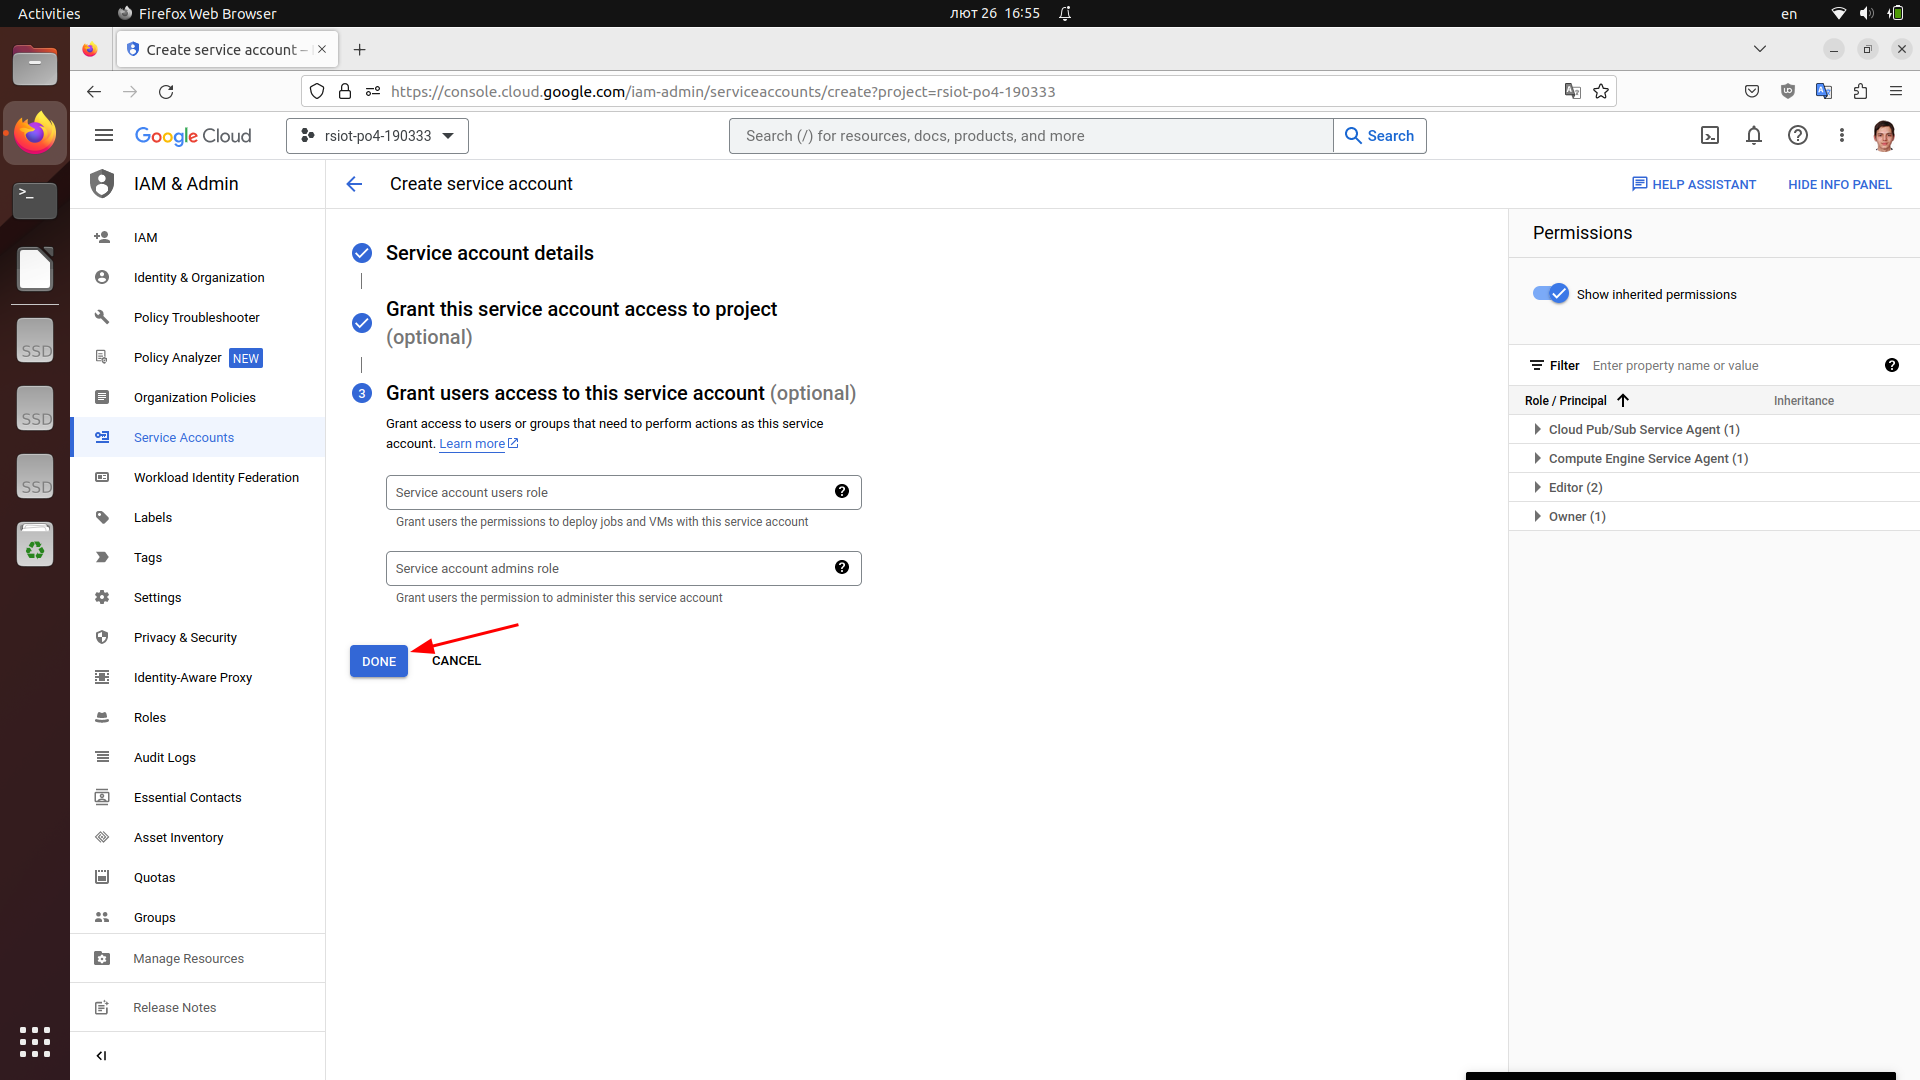
\includegraphics[width=11cm]
    {images/2023-02-26_16-56-00.png}
    \caption{\_}
    \label{fig:9}
  \end{figure}

  Жмём по созданой почте (см. рисунок~\ref{fig:10}).

  \begin{figure}[!h]
    \centering
    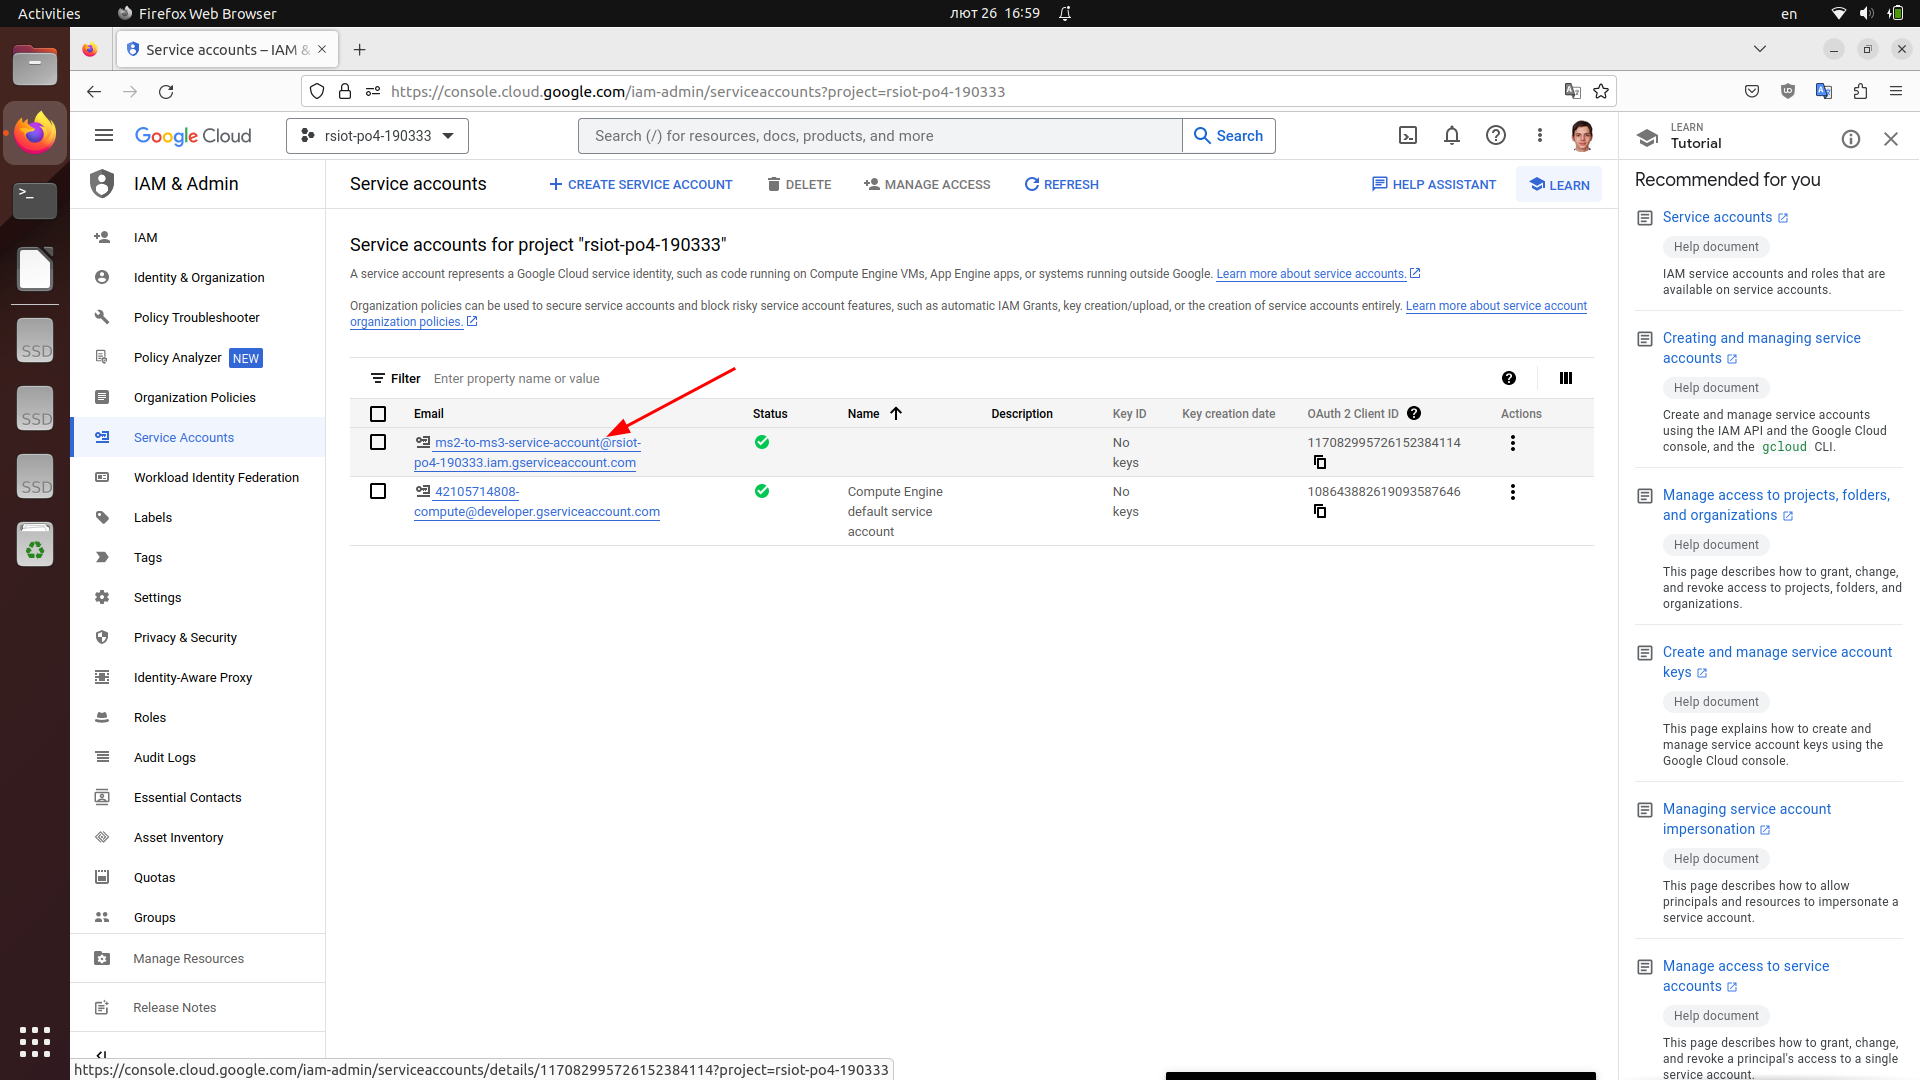
\includegraphics[width=11cm]
    {images/2023-02-26_16-59-46.png}
    \caption{\_}
    \label{fig:10}
  \end{figure}

  Жмём <<KEYS>> (см. рисунок~\ref{fig:11}).

  ADD KEY > Create new key (см. рисунок~\ref{fig:11}).

  Жмём <<JSON>> (см. рисунок~\ref{fig:12}).

  Жмём <<CREATE>> (см. рисунок~\ref{fig:12}).

  \begin{figure}[!h]
    \centering
  
    \begin{minipage}{0.49\textwidth}
      \centering
  
      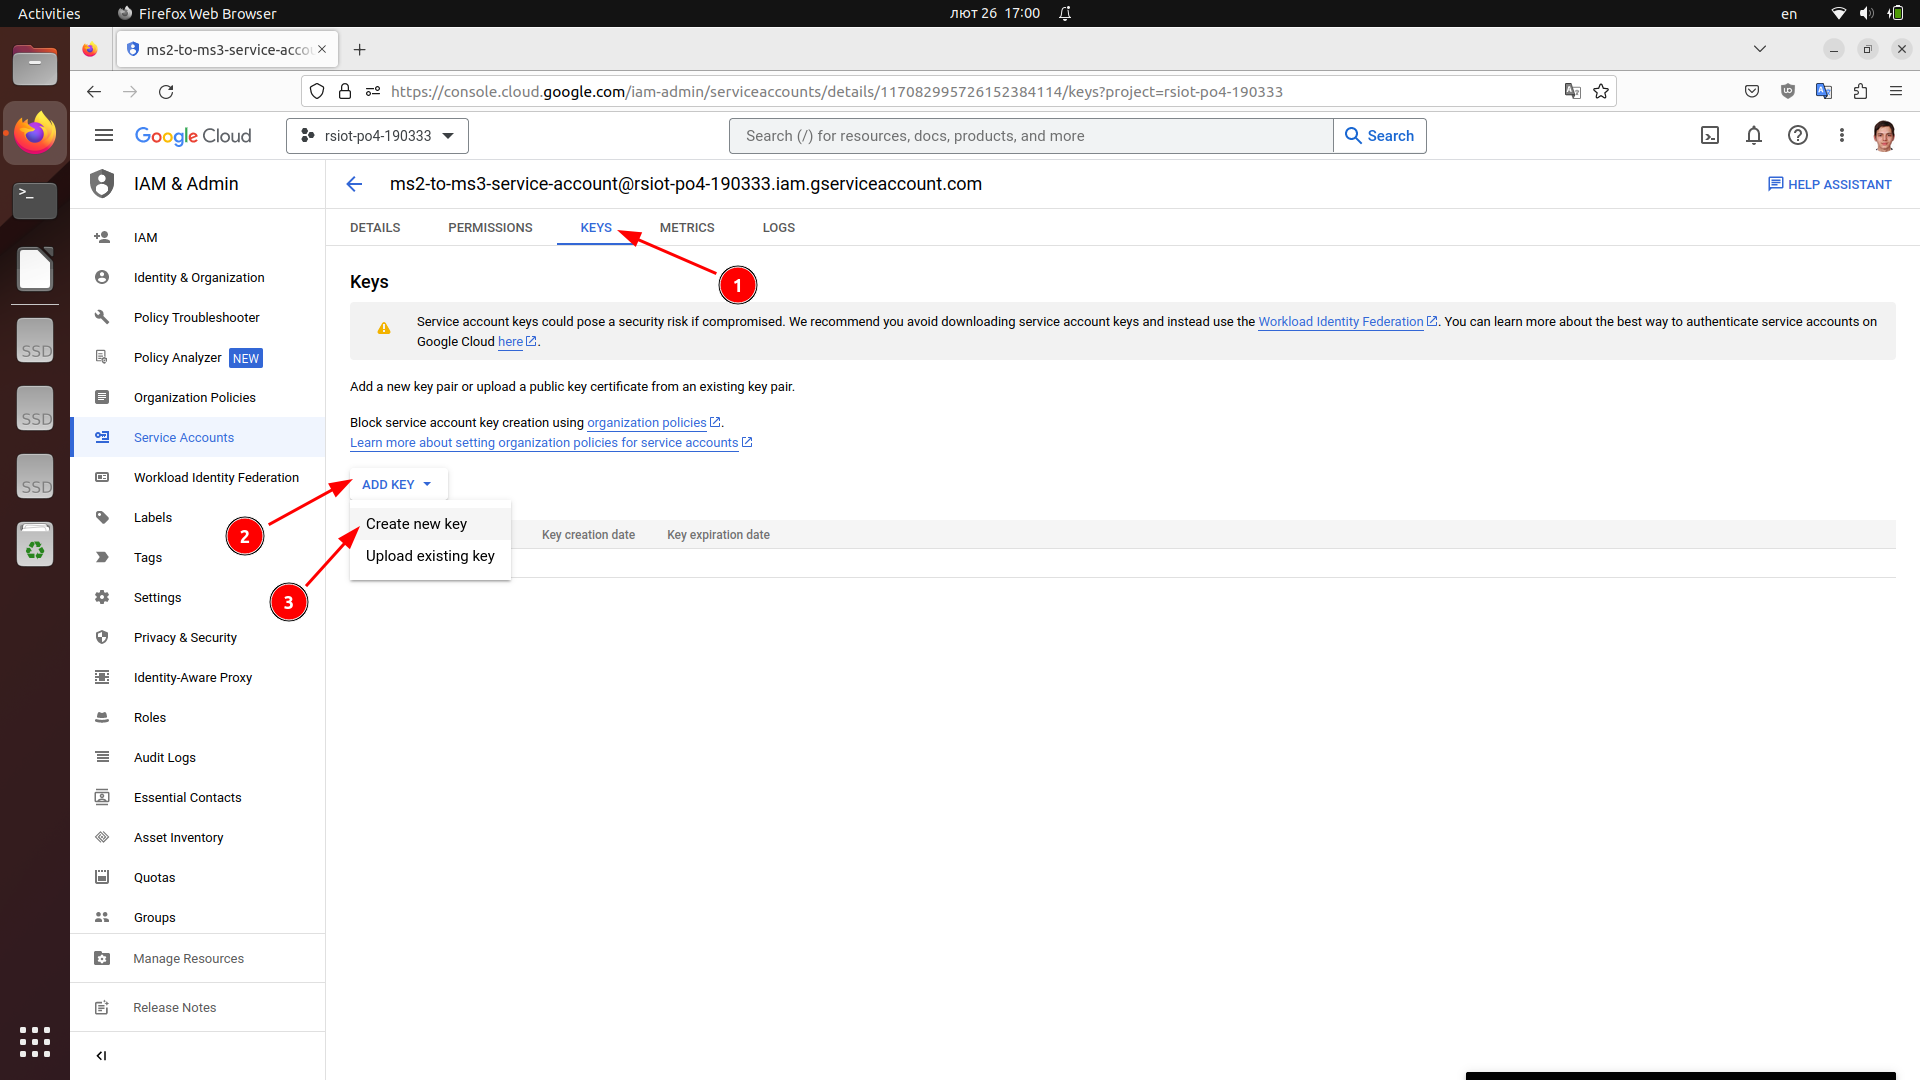
\includegraphics[height=5cm]
      {images/2023-02-26_17-00-46.png}
  
      \caption{\_}
  
      \label{fig:11}
    \end{minipage}
    \begin{minipage}{0.49\textwidth}
      \centering
  
      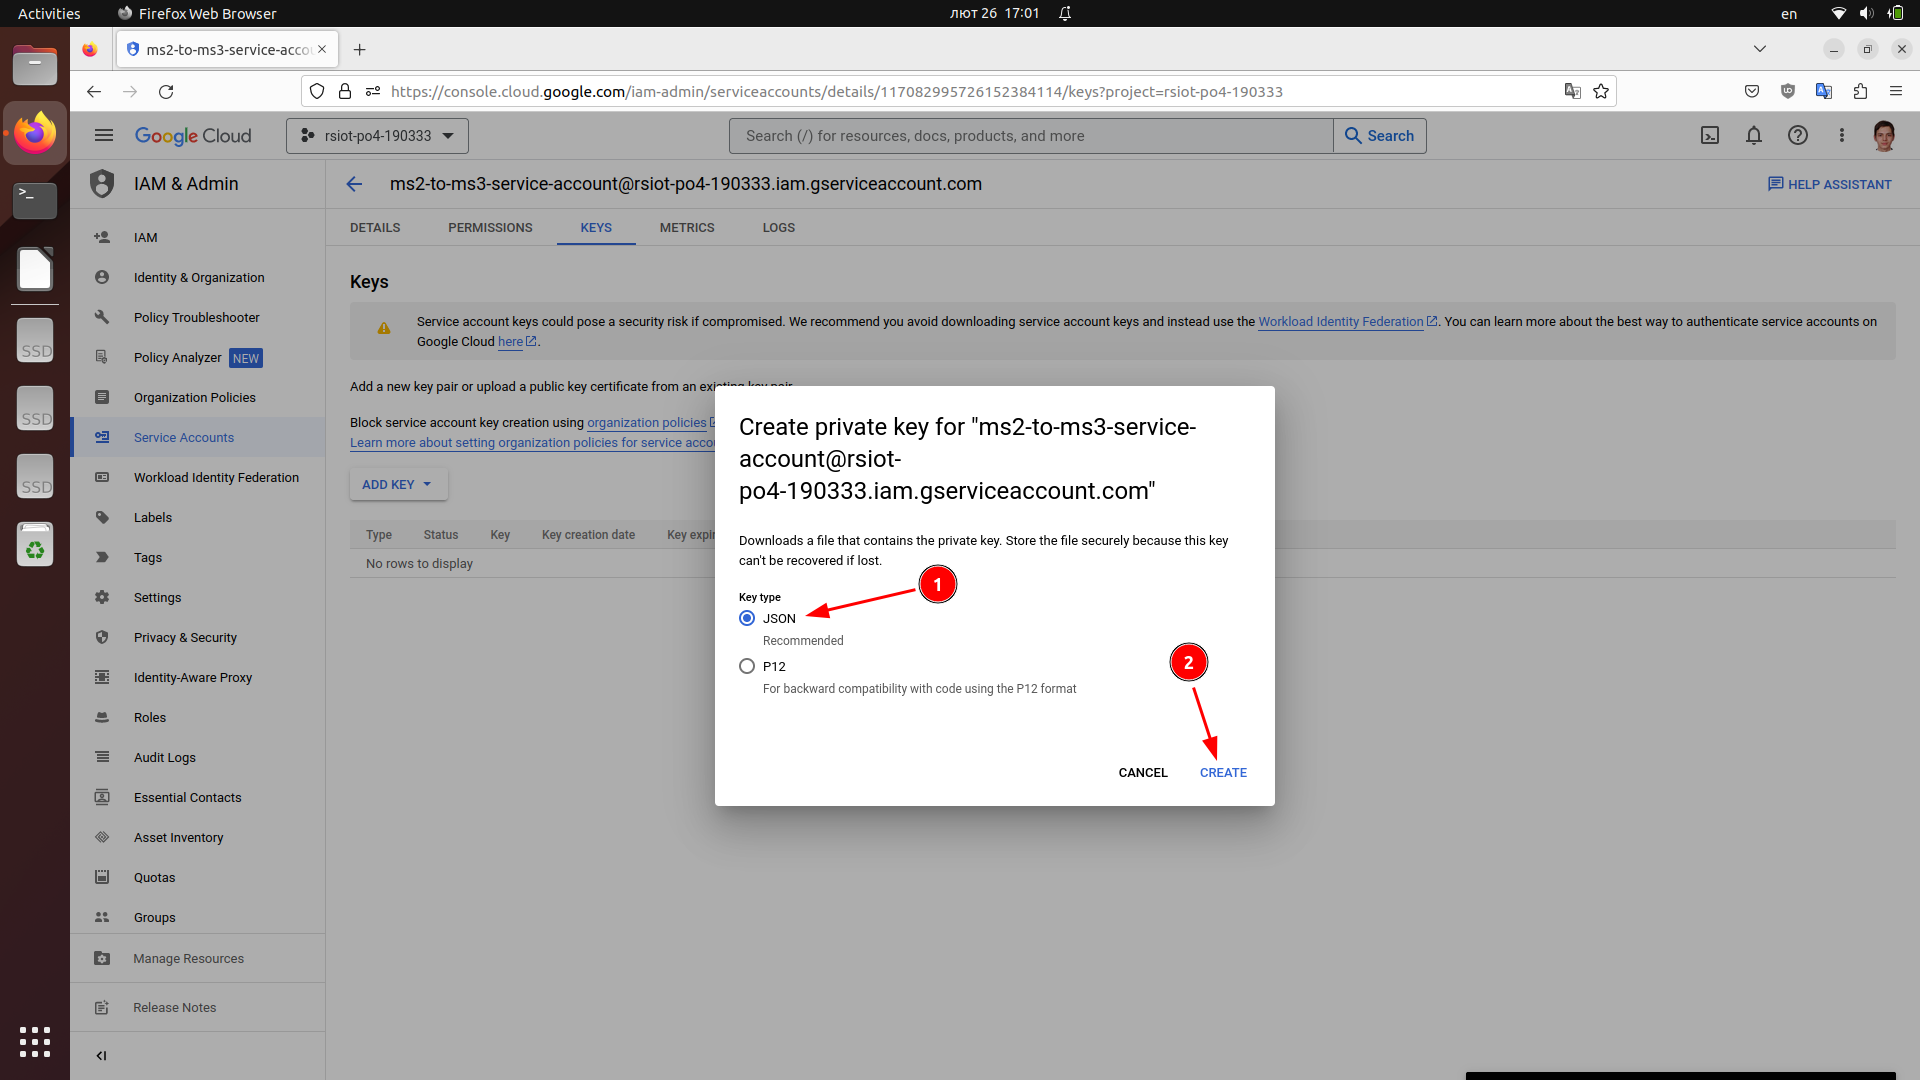
\includegraphics[height=5cm]
      {images/2023-02-26_17-01-18.png}
  
      \caption{\_}
  
      \label{fig:12}
    \end{minipage}
  \end{figure}

  \newpage

  \lstinputlisting[]{../sources/MS2/dev.env.example}

  \lstinputlisting[language=Java]{../sources/MS2/src/main.ts}

  \lstinputlisting[]{../sources/MS3/dev.env.example}

  \lstinputlisting[language=Java]{../sources/MS3/src/app.js}

  \newpage

  \begin{lstlisting}[language=bash,name=Загрузка MS3 на Google Cloud App Engine]
    gcloud projects list
    gcloud config set project rsiot-po4-190333
    gcloud app create
    gcloud app deploy app.yaml
    gcloud app browse
    gcloud app describe
  \end{lstlisting}

  \begin{lstlisting}[language=bash,name=Обновление MS3 на Google Cloud App Engine]
    gcloud app deploy app.yaml
    gcloud app browse
    gcloud app describe
  \end{lstlisting}

  % \newpage

  \begin{lstlisting}[name=Создаём статью микроблога]
    curl -X 'POST' \
      'http://34.173.23.213/api/posts' \
      -H 'accept: application/json' \
      -H 'Content-Type: application/json' \
      -d '{
      "userId": 1,
      "title": "С Новым годом!",
      "content": "Отмечается в ночь с 31 декабря по 1 января."
    }'
  \end{lstlisting}

  \begin{lstlisting}[name={Если от MS3 к MS2 пришел true, то MS2 вернёт JSON}]
    {
      "userId": 1,
      "title": "С Новым годом!",
      "content": "Отмечается в ночь с 31 декабря по 1 января.",
      "id": 1
    }
  \end{lstlisting}

  \begin{lstlisting}[name={Если от MS3 к MS2 пришел false, то MS2 вернёт JSON}]
    {
      "statusCode": 400,
      "message": "MS3 решил не выполнять запрос"
    }
  \end{lstlisting}

  \begin{lstlisting}[name={Если (за 4000 милисекунд) не успел прийти ответ, то MS2 вернёт JSON}]
    {
      "statusCode": 400,
      "message": "MS3 не ответил в течение заданного времени.",
      "more": {
        "message": "MS3 запущен и работает!"
      }
    }
  \end{lstlisting}

  \newpage

  \paragraph{} \textbf{Вывод}:
  Создали темы PubSub. Создали подписчиков для тем PubSub. Написали MS3, который читает сообщения из PubSub, которые отправил MS2.
  MS3 генерирует с вероятностью 50\% ответ положительный. Отредактировали MS2.
  Если на MS2 приходит отрицательный ответ, то это 400, иначе запрос выполнения эндпоинта разрешен.
  Выложили MS3 на Google Cloud App Engine. Выложили MS2 на Google Cloud Compute Engine.
  
  % = = = = = = = = = = = = = = = =
  % \newpage
  \begingroup
    \phantomsection
    \addcontentsline{toc}{section}{СПИСОК ИСПОЛЬЗОВАННЫХ ИСТОЧНИКОВ}
    \section*{Список использованных источников} %\section*{СПИСОК ИСПОЛЬЗОВАННЫХ ИСТОЧНИКОВ}

    \renewcommand{\addcontentsline}[3]{}% Remove functionality of \addcontentsline
    \renewcommand{\section}[2]{}% Remove functionality of \section

    \begin{thebibliography}{}

    \bibitem{YouTube_PubSub}
    Set up \& use PubSub with Python - YouTube
    [Electronic resource]. -
    Mode of access:
    \url{https://www.youtube.com/watch?v=xOtrCmPjal8}.
    Date of access: 16.02.2023.

    \bibitem{GoogleCloudConsole}
    Welcome – Google Cloud console
    [Electronic resource]. -
    Mode of access:
    \url{https://console.cloud.google.com/welcome}.
    Date of access: 26.02.2023.

    \bibitem{GoogleCloudPubSubTopic}
    Topics – Pub/Sub – Google Cloud console
    [Electronic resource]. -
    Mode of access:
    \url{https://console.cloud.google.com/cloudpubsub/topic/list}.
    Date of access: 26.02.2023.

    \bibitem{GoogleCloudPubSubSubscriptions}
    Subscriptions – Pub/Sub – Google Cloud console
    [Electronic resource]. -
    Mode of access:
    \url{https://console.cloud.google.com/cloudpubsub/subscription/list}.
    Date of access: 26.02.2023.

    \bibitem{GoogleCloudServiceAccount}
    Service accounts – IAM \& Admin – Google Cloud console
    [Electronic resource]. -
    Mode of access:
    \url{https://console.cloud.google.com/iam-admin/serviceaccounts}.
    Date of access: 26.02.2023.

  \end{thebibliography}
  \endgroup
  % = = = = = = = = = = = = = = = =
\end{document}
